%!TEX root = seminar_yw_full.tex

% Font and math symbols
\usepackage{amsmath,amsfonts,amssymb}
\usepackage{xspace}
\def\SSS{\mathcal{S}}
\def\FFF{\mathcal{F}}
\def\NominalP{Nominal\texttt{+}\xspace}
\def\NominalPP{Nominal\texttt{++}\xspace}

\iffontsavailable{Iosevka}{%
    \setmonofont[BoldFont={Iosevka Bold Extended},%
        ItalicFont={Iosevka Italic},%
        BoldItalicFont={Iosevka Bold Extended Italic},%
        Contextuals=Alternate]{Iosevka Extended}%
}{}

% \iffontsavailable{Helvetica}{%
%     \setsansfont{Helvetica}%
% }{}

% Sub-equations with large bracket
\usepackage{cases}

% itemized margin
\setlength\leftmargini{2pt}
\setbeamertemplate{itemize item}{\indent}

% Tables
\usepackage{booktabs}
\usepackage{threeparttable}

% Units and decimal point alignment
\usepackage[per-mode=symbol, range-phrase=\textendash, range-units = single, detect-all]{siunitx}
\DeclareSIUnit\bit{b}
\DeclareSIUnit\fiber{fiber}
\DeclareSIUnit\channel{channel}
\DeclareSIUnit\group{group}
\DeclareSIUnit\bps{bps}
\DeclareSIUnit\dbm{dBm}

% Chemical formula
\usepackage{chemformula}

% Various markers
\usepackage{pifont}
\newcommand{\cmark}{\ding{51}}%
\newcommand{\xmark}{\ding{55}}%
\newcommand{\done}{\rlap{$\square$}{\raisebox{2pt}{\large\hspace{1pt}\cmark}}%
    \hspace{-2.5pt}}
\newcommand{\wontfix}{\rlap{$\square$}{\large\hspace{1pt}\xmark}}

% Centered text box
\usepackage{varwidth}

\usepackage{transparent}

% choose bibliography style for formatting list of publications
\usepackage[style=nature,url=false,doi=false,maxbibnames=99,backend=biber]{biblatex}
\DeclareFieldFormat{labelnumberwidth}{\textup{\texttt{[#1]}}}
\AtEveryCitekey{\clearfield{issn}}
\AtEveryCitekey{\clearfield{title}}
\AtEveryCitekey{\clearfield{publisher}}
\AtEveryCitekey{\clearfield{address}}
\renewcommand*{\bibfont}{\tiny}

% Absolute path
\usepackage{currfile-abspath}
\getmainfile % get real main file (can be different than jobname in some cases)
\getabspath{\themainfile} % or use \jobname.tex instead (not as safe)
\let\mainabsdir\theabsdir % save result away (macro will be overwritten by the next \getabspath
\let\mainabspath\theabspath % save result away (macro will be overwritten by the next \getabspath

\usepackage{bm}
\usepackage{soul}
\soulregister\emph7
\soulregister\textbf7
\soulregister\textendash7
\bibliography{\mainabsdir../../../9_interview/0_slides_common/papers}
% \nocite{*}

\title{Photonics-Empowered Computing}
\subtitle{From Efficient to Functional Data Movement}

\date{February 13, 2025}
\author{Yuyang~Wang}
\institute{
    \begin{tabular}{@{}r@{}@{\hskip1pt}l@{}}
        &\emph{Postdoctoral Research Scientist, Columbia Nano Initiative}\\
        &Columbia University in the City of New York, New York, NY 10027\\
        &\email{yw3831@columbia.edu}
    \end{tabular}
}
\cornergraphic{\mainabsdir../../../9_interview/0_slides_common/figures/CU/CU_Corner.jpg}
\leftlogo{\mainabsdir../../../9_interview/0_slides_common/figures/CU/Columbia_University_Logo-white.eps}
\rightlogo{\mainabsdir../../../9_interview/0_slides_common/figures/CU/LRL_Logo_white.png}
\institutelogo{\mainabsdir../../../9_interview/0_slides_common/figures/CU/Columbia_Engineering_Two_Tone.eps}

\setbeamertemplate{frame footer left}{\insertsectionsubsectionhead}
\setbeamertemplate{frame footer middle}{ASU ECEE Seminar}
\setbeamertemplate{frame footer right}{\usebeamertemplate*{frame numbering}}

\begin{document}

\maketitle
\lrlset{sectionpage=none}

%!TEX root = ../research_overview.tex

\section{Grand Challenge}

\subsection{Energy Cost Limiting Scalability}

\begin{frame}{AI Applications Driving Explosive Growth}

    \only<2-2|handout:0>{\centering\includegraphics[width=0.6\textwidth]{fig/model_growth-1_compressed.pdf}}%
    \only<3-3|handout:0>{\centering\includegraphics[width=0.6\textwidth]{fig/model_growth-2_compressed.pdf}}%
    \only<4-4>{\centering\includegraphics[width=0.6\textwidth]{fig/model_growth-3_compressed.pdf}}%
    \vspace{-1em}%
    \begin{center}%
        \onslide<2->{\fullcite{wuPetaScaleEmbeddedPhotonics2023}}%
    \end{center}%
    \note<1-1>[item]{We all know that Moore's Law is slowing down and coming to an end.}
    \note<2-2>[item]{But the growth of computational demand is not. This is especially driven by the explosive growth of AI applications.}
    \note<2-2>[item]{As we can see here, the size of AI models has been growing nearly an order of magnitude per year over the past six to eight years, and the largest model has already exceeded 100 trillion parameters. As a result, there is simply no way to fit these models into any single computing unit.}
    \note<3-3>[item]{And people have known this for a while, and that's why there has been tremendous effort from the computer engineering side to program around data locality, knowing that long-distance data movement is very expensive.}
    \note<4-4>[item]{But as these models grow larger and larger, long-distance communications are becoming unavoidable in the computation of these workloads.}
    \note<4-4>[item]{So, if these communications cannot be done in a more efficient way,}

\end{frame}

\begin{frame}{Per-Training Energy Consumption}

    \only<1-1|handout:0>{\centering\includegraphics[width=0.8\textwidth]{fig/energy_growth-1_compressed.pdf}}%
    \only<2-2|handout:0>{\centering\includegraphics[width=0.8\textwidth]{fig/energy_growth-2_compressed.pdf}}%
    \only<3-3|handout:0>{\centering\includegraphics[width=0.8\textwidth]{fig/energy_growth-3_compressed.pdf}}%
    \only<4-4>{\centering\includegraphics[width=0.8\textwidth]{fig/energy_growth-4_compressed.pdf}}%
    \vspace{-1em}%
    \begin{center}%
        \fullcite{liangHolisticEvaluationLanguage2023,pattersonCarbonEmissionsLarge2021,masanetRecalibratingGlobalData2020}%
    \end{center}%
    \note<1-1>[item]{we will see this tremendous growth in the energy consumption of these workloads to continue surging in an unsustainable way.}
    \note<2-2>[item]{For example, GPT-4, which is marked on the top right corner, is estimated to be trained on 25 thousand GPUs, costing over 51 thousand megawatt-hours of energy, and it takes over 3 months to finish the training.}
    \note<3-3>[item]{And just to put it in some perspective, this megawatt-hour number for training a single AI model is greater than the hourly electricity used by the entire New York City in a hot summer day.}
    \note<4-4>[item]{So, this energy cost has really become environmentally significant, and is preventing the system from being able to scale and support a wide range of real-world applications, like climate prediction, drug discovery, financial modeling, digital twins, and defense applications.}
    \note<4-4>[item]{So, large-scale computing systems nowadays are really about computation AND communication. But what exactly is the problem with today's data communication technologies?}


\end{frame}

\subsection{Communication Bottleneck}

\begin{frame}{Challenges Moving Data Off-Chip}
    \only<2-2|handout:0>{\centering\includegraphics[width=\textwidth]{fig/bw_taper-1_compressed.pdf}}%
    \only<3-3|handout:0>{\centering\includegraphics[width=\textwidth]{fig/bw_taper-2_compressed.pdf}}%
    \only<4-4|handout:0>{\centering\includegraphics[width=\textwidth]{fig/bw_taper-3_compressed.pdf}}%
    \only<5-5|handout:0>{\centering\includegraphics[width=\textwidth]{fig/bw_taper-4_compressed.pdf}}%
    \only<6-6>{\centering\includegraphics[width=\textwidth]{fig/bw_taper-5_compressed.pdf}}%
    \note<1-1>[item]{Let's take a look at a major bottleneck in today's systems, which is the communication bottleneck. And many have referred to it as the interconnect bottleneck, or the memory wall in a slightly different context.}
    \note<2-2>[item]{More specifically, in today's systems, data from one computing node needs to travel across several levels of network hierarchy to reach another computing node.}
    \note<3-3>[item]{When this data is moved within the socket, like between the GPU and the memory, we see that the bandwidth there is actually tremendous, up to several terabytes per second. And the energy efficiency is REALLY great, in the order of femtojoules per bit. This bandwidth and energy efficiency are achieved by using very dense and parallel electrical interconnects, like a highway for digital data with many many lanes.}
    \note<4-4>[item]{But this ultra-efficient data movement doesn't go very far. As we move to the board level, and look between the GPUs, we see that the bandwidth drops by a factor of 5 or so, because the signals need to travel a bit longer in distance and perhaps through a switch fabric. But it is still quite good, well above 1 terabyte per second in those best-in-class commercial solutions. And the energy consumption is about tens to hundreds of femtojoules per bit, which is still not bad.}
    \note<5-5>[item]{What really becomes dramatic is when the data needs to go off-board and travel several meters or even hundreds of meters across the data center. This is where the bandwidth plunges to below 1 tera BIT per second. Note it is not byte here. This is also where traditionally optical communication starts to get used, in the form of pluggable optical transceivers, but they are nowhere near being energy efficient, usually consuming more than 20 PICOjoules per bit.}
    \note<6-6>[item]{So it's really like having a superhighway of data that suddenly narrows down to a dirt road. And because of this, we are seeing a two order of magnitude, maybe even more, bandwidth discrepancy across the network hierarchy. And these long-distance links are consuming too much energy to provide not even enough bandwidth, which further slows down the application execution and leads to even more energy consumption spent on computation because of the prolonged execution time.}
    \note<6-6>[item]{Now, how can we use integrated photonics to address this bandwidth and energy problem?}

\end{frame}
%!TEX root = ../research_overview.tex

\section{Embedded Photonics}

\subsection{Concept}

\begin{frame}{Bringing Photonics into Computing Sockets}

    \only<2-2|handout:0>{\centering\includegraphics[width=0.8\textwidth]{fig/cpo-1_compressed.pdf}}%
    \only<3-3>{\centering\includegraphics[width=0.8\textwidth]{fig/cpo-2_compressed.pdf}}%
    \note<1-1>[item]{My approach is to bring photonic technologies into the computing sockets.}
    \note<2-2>[item]{If we look at today's pluggable optical transceivers, we see these long electrical wires, which can be up to tens of centimeters, that are still needed between the computing chip and the optical interface. To drive these electrical wires at something like 100 Gb/s is where the energy efficiency really starts to degrade.}
    \note<3-3>[item]{So, my research has focused on integrating the photonics data input/output directly into the computing socket, because once the data is in the optical domain, the bandwidth and energy become virtually independent of distance, which means it can travel either centimeters or hundreds of meters with roughly the same bandwidth and energy efficiency. So the key is to really have this electrical to optical conversion happen as close as possible to where the data is generated.}
    \note<3-3>[item]{So, for those of you that have learned about my research on zoom,}
    % \note<3-3>[item]{But this is very challenging, because we are building a system, and we not only need to figure out the integration and packaging strategies, which I'll talk about later, but we also need to find the optimal design for the photonics part that seamlessly interface to the electronics.}

\end{frame}

\subsection{Impact}

\begin{frame}{What System-Level Impact?}
    \only<2-2|handout:0>{\centering\includegraphics[width=\textwidth]{fig/sipam-1_compressed.pdf}}%
    \only<3-3|handout:0>{\centering\includegraphics[width=\textwidth]{fig/sipam-2_compressed.pdf}}%
    \only<4-4>{\centering\includegraphics[width=\textwidth]{fig/sipam-3_compressed.pdf}}%
    \note<1-1>[item]{I'd like to bring your attention to this system-level study that I didn't mention, which is really trying to see what can be potentially achieved if we have this ultra-high bandwidth delivered right to the computing socket.}
    \note<2-2>[item]{Imagine we equip this state-of-the-art GPU, which has a shoreline of roughly 24 mm, with optical I/O that provides, say, 4 Tb/s/mm bandwidth density. This is equivalent to having a 96 Tb/s, or 12 terabyte per second, bidirectional bandwidth that can reach any distance within the system.}
    \note<3-3>[item]{What this would allow for is a fully disaggregated system where all memory units are in a remote pool, but can be treated as if they are local to the GPU. We then used a tool called Calculon, which is actually co-authored by Nvidia and Georgia Tech, to evaluate some Transformer-based workloads on this system architecture,}
    \note<4-4>[item]{and we were delighted to see that we might potentially get a 5 to 7x speedup in the execution time of these workloads, compared to a baseline system using Nvidia H100 GPUs interconnected with NVLinks.}
    \note<4-4>[item]{So, can we make an optically connected compute socket like this? My answer is yes. But, this is a very challenging task, because we not only need to figure out the integration and packaging details, which I'll talk about later, but we also need to find the optimal design for the photonics part that seamlessly interface to the electronics.}

\end{frame}

\subsection{Approach}

\begin{frame}{``Going Fast by Going (Wide and) Slow''}

    \only<2-2|handout:0>{\centering\includegraphics[width=0.8\textwidth]{fig/fom-1_compressed.pdf}}%
    \only<3-3|handout:0>{\centering\includegraphics[width=0.8\textwidth]{fig/fom-2_compressed.pdf}}%
    \only<4-4|handout:0>{\centering\includegraphics[width=0.8\textwidth]{fig/fom-3_compressed.pdf}}%
    \only<5-5>{\centering\includegraphics[width=0.8\textwidth]{fig/fom-4_compressed.pdf}}%
    \note<1-1>[item]{And, one example of this photonic-electronic co-design is to figure out how many parallel wavelength channels we need to have in each link to achieve the target bandwidth with the best energy efficiency.}
    \note<2-2>[item]{So, what I'm about to show here is a combined metric of bandwidth density and energy efficiency, where the x-axis is the number of parallel wavelength channels needed for 1 Tb/s bandwidth. In other words, to the left of the x-axis, there are fewer wavelength channels, each operating at a higher data rate, and to the right, there are more wavelength channels, each operating at a lower data rate.}
    \note<3-3>[item]{And, here are some data points I collected from existing solutions, either commercial or research. And we see that the link metric sort of plateaus for various configurations, even for the best-in-class commercial solutions like those from Intel and AyarLabs.}
    \note<4-4>[item]{And what my work was able to achieve, through the exploration of this design space and optimizing the photonics design, is to improve this metric by two orders of magnitude. And there were two key factors that contributed to this improvement.}
    \note<5-5>[item]{One is the use of a moderate data rate per channel, for which I found a sweet spot between 16 and 32 Gb/s, which really saves energy from the electronic driver and receiver circuitry; and the second is to really increase the number of parallel wavelength channels we can have in one link, from today's less than 16, to something like 64 and beyond.}

\end{frame}
%!TEX root = ../research_overview.tex

\section{Scalable Architecture}

\subsection{Comb-Driven DWDM}

\begin{frame}{Massive Wavelength Parallelism}

    \only<2-2|handout:0>{\centering\includegraphics[width=0.9\textwidth]{fig/dwdm-1_compressed.pdf}}%
    \only<3-3|handout:0>{\centering\includegraphics[width=0.9\textwidth]{fig/dwdm-2_compressed.pdf}}%
    \only<4-4|handout:0>{\centering\includegraphics[width=0.9\textwidth]{fig/dwdm-3_compressed.pdf}}%
    \only<5-5>{\centering\includegraphics[width=0.9\textwidth]{fig/dwdm-4_compressed.pdf}}%
    \vspace{-1em}%
    \begin{center}%
        \onslide<4->{\fullcite{kimTurnkeyHighefficiencyKerr2019}\quad\quad\quad\quad}%
        \onslide<5->{\fullcite{rizzoPetabitScaleSiliconPhotonic2023}}%
    \end{center}%
    \note<1-1>[item]{Now let me talk about how I was able to greatly expand the number of wavelength channels in a single link beyond 64.}
    \note<2-2>[item]{And I'll first show a canonical wavelength-division multiplexing architecture based on a photonic device called microresonators.}
    \note<2-2>[item]{So, wavelength-division multiplexing, or WDM, is a well-known advantage of doing optical signaling, because we can have multiple wavelengths, or colors of light if you will, carrying different streams of data and propagating in the same waveguide or fiber.}
    \note<2-2>[item]{And then, what's unique about these microresonator modulators is that they achieve two functions with one device: first, they select a wavelength, and then you can modulate them electrically to encode data onto that wavelength. So, by having a series of these devices cascaded along the same waveguide, and each of them designed to select a different wavelength, you can modulate these wavelengths independently and virtually without affecting one another.}
    \note<2-2>[item]{The receiver side is kinda similar, but with microresonator filters to separate the wavelengths onto individual photodetectors.}
    \note<2-2>[item]{But if you take a look at what's available out there, you'll probably find that none of those existing WDM transceivers actually used more than 16 wavelengths.}
    \note<3-3>[item]{This is because, one of the biggest challenges is to have a multi-wavelength optical source. And for a channel count as high as 64, this simply cannot be done using an individual laser for each wavelength, because of the packaging and control complexities and the power consumption.}
    \note<4-4>[item]{So, one of the key enabling technologies that my research leverages is a Kerr frequency comb source. It is a device that uses the non-linear Kerr effect in Silicon Nitride to generate potentially more than a hundred wavelength channels from a single laser. And these channels will have a precise intrinsic spacing that doesn't require any additional control on a per-channel basis.}
    \note<5-5>[item]{And then, I co-designed the photonics link with this comb source, using a scalable link architecture that features this unique topology with multiple buses. What it does is that, instead of having a single bus waveguide that cascades all of the microresonators, which would of course lead to significant crosstalk and accumulated insertion loss because we are talking about 64 channels or more, it subdivides the comb channels into multiple groups, using these special de-interleaving structures, and each group is modulated by a separate bank of modulators.}
    \note<5-5>[item]{This way, both the crosstalk and the accumulated insertion loss are significantly reduced, because with each stage of de-interleaving, the effective channel spacing on each bus is doubled, and the number of resonators is halved.}

\end{frame}

\subsection{Tb/s-Class Link Design}

\begin{frame}{Tb/s per Fiber Link Co-Designed with Comb}

    \only<2-2|handout:0>{\centering\includegraphics[width=0.9\textwidth]{fig/arch-1_compressed.pdf}}%
    \only<3-3|handout:0>{\centering\includegraphics[width=0.9\textwidth]{fig/arch-2_compressed.pdf}}%
    \only<4-4|handout:0>{\centering\includegraphics[width=0.9\textwidth]{fig/arch-3_compressed.pdf}}%
    \only<5-5|handout:0>{\centering\includegraphics[width=0.9\textwidth]{fig/arch-4_compressed.pdf}}%
    \only<6-6|handout:0>{\centering\includegraphics[width=0.9\textwidth]{fig/arch-5_compressed.pdf}}%
    \only<7-7|handout:0>{\centering\includegraphics[width=0.9\textwidth]{fig/arch-6_compressed.pdf}}%
    \only<8-8|handout:0>{\centering\includegraphics[width=0.9\textwidth]{fig/arch-7_compressed.pdf}}%
    \only<9-9|handout:0>{\centering\includegraphics[width=0.9\textwidth]{fig/arch-8_compressed.pdf}}%
    \only<10-10>{\centering\includegraphics[width=0.9\textwidth]{fig/arch-9_compressed.pdf}}%
    \note<1-1>[item]{Now, let me show you some details of my link design that achieves a Tb/s data rate per fiber.}
    \note<2-2>[item]{The link starts from a comb source with 100 GHz channel spacing, which is roughly 0.8 nm in the 1550 nm C-band. It can generate more than 70 channels that are above half a mW of optical power.}
    \note<3-3>[item]{On the transmitter side, I chose to use two stages of de-interleavers to divide the comb channels onto four buses. Each bus has 16 microresonator modulators that can modulate 16 comb lines independently. And then, the modulated signals are recombined and coupled into a single-mode fiber.}
    \note<4-4>[item]{On the receiver side, a symmetric architecture is used to separate the channels and detect them with photodetectors.}
    \note<5-5>[item]{The beauty of this link architecture is that, it can achieve an aggregate data rate of 1 Tb/s per fiber, requiring only a modest 16 Gb/s data rate per channel. And it is highly scalable, because it allows for using a comb spectrum that is much wider than the resonator free-spectral range.}
    \note<6-6>[item]{Let me show you what that means. As we can see here, a resonator doesn't have only one resonance. In fact, it has a series of resonances that are spaced by its free-spectral range, or FSR. So, when we're designing the links, we really need to co-design the resonator FSR with the comb, so that these unwanted resonances don't overlap with any other comb lines on the bus.}
    \note<7-7>[item]{Fortunately, we have a closed-form solution to achieve this, and we call it the multi-FSR channel arrangement. And what's cool about it is that, we can design the FSR so that we may arrange more than 16 resonators on a bus, without having channel conflicts, for example, 17 as in this configuration, or even 19 if we use a slightly larger FSR. This flexibility gives us some redundancy just in case there are bad comb lines or resonators after fabrication.}
    \note<8-8>[item]{And finally, this is how the channel arrangement looks like on all four buses.}

\end{frame}

\subsection{Link Validation}

\begin{frame}{End-to-End Link Validation}

    \only<2-2|handout:0>{\centering\includegraphics[width=0.8\textwidth]{fig/validation-1_compressed.pdf}}%
    \only<3-3|handout:0>{\centering\includegraphics[width=0.8\textwidth]{fig/validation-2_compressed.pdf}}%
    \only<4-4|handout:0>{\centering\includegraphics[width=0.8\textwidth]{fig/validation-3_compressed.pdf}}%
    \only<5-5>{\centering\includegraphics[width=0.8\textwidth]{fig/validation-4_compressed.pdf}}%
    \vspace{-1em}%
    \begin{center}%
        \onslide<2->{\fullcite{wangCoDesignedSilicon2024}}%
    \end{center}%
    \note<1-1>[item]{To validate this link architecture,}
    \note<2-2>[item]{I designed this photonic test chip, which was fabricated through AIM Photonics.}
    \note<2-2>[item]{This chip contains the exact same 4 by 17 modulator and filter arrays as I just described in the architecture.}
    \note<3-3>[item]{And I conducted data transmission experiments with comb input, where the comb spectrum is shown here.}
    \note<4-4>[item]{In the test setup, I used one test chip as the transmitter and another as the receiver.}
    \note<5-5>[item]{And what I'm showing here are the eye diagrams gathered from 10 channels, each operating at 16 Gb/s. These open eyes demonstrate the feasibility of the link architecture to utilize the massive number of wavelengths from the Kerr comb source.}

\end{frame}

%!TEX root = ../research_overview.tex

\section{Integration and Packaging}

\subsection{Approach}

\begin{frame}{Hybrid 2.5D/3D Integration}

    \only<2-2|handout:0>{\centering\includegraphics[width=0.8\textwidth]{fig/integration-1_compressed.pdf}}%
    \only<3-3>{\centering\includegraphics[width=0.8\textwidth]{fig/integration-2_compressed.pdf}}%
    \note<1-1>[item]{So, that was the link design. To get the bandwidth density though, we need to think about how to integrate the photonics with electronic drivers and package with the compute chip.}
    \note<2-2>[item]{What I'm showing here are some of the integration and packaging options. And together with Cornell University and Intel,}
    \note<3-3>[item]{we made the first demonstration of a co-packaged optical I/O assembly that takes the bottom-right approach, which is a hybrid 2.5D/3D integration.}
    \note<3-3>[item]{More specifically, we developed a multi-chip package, or MCP, that has the photonic chiplet and electronic chiplet stacked on top of each other, and then this sub-assembly is further integrated with the compute chip through a silicon interposer.}
    \note<3-3>[item]{Compared to other approaches that use a monolithic chiplet for both photonic components and their electronic drivers, having two separate chiplets for photonics and electronics allows us to optimize both using different process nodes, and also achieve a much higher density by using flip-chip bonding with a smaller microbump pitch.}
    \note<3-3>[item]{And the 2.5D integration with the compute chip requires no changes to the compute chip itself, which is a big advantage for system prototyping.}

\end{frame}

\subsection{Multi-Chip Package}

\begin{frame}{96\,Tb/s Multi-Chip Package}

    \only<1-1|handout:0>{\centering\includegraphics[width=\textwidth]{fig/mcp-1_compressed.pdf}}%
    \only<2-2>{\centering\includegraphics[width=\textwidth]{fig/mcp-2_compressed.pdf}}%
    \vspace{-1em}%
    \begin{center}%
        \onslide<1->{\fullcite{wangCoDesignedSilicon2024}}%
    \end{center}%
    \note<1-1>[item]{So, here's what the multi-chip package looks like. And I actually have one here, so you can get an idea of how large it is.}
    \note<2-2>[item]{Inside the package, there is an Intel FPGA that acts as the compute chip, and three of these photonic-electronic sub-assemblies co-integrated through Intel's EMIB technology.}
    \note<2-2>[item]{And this MCP is designed to provide a 96 Tb/s bidirectional bandwidth into and out of the package, and I'll show you how this number is achieved.}

\end{frame}

\begin{frame}{4\,Tb/s/mm Shoreline Bandwidth Density}

    \note<1-1>[item]{Here is what it looks like under the hood. In this collaborative work, I designed the three photonic chips, each bonded to an electronic driver chip designed at Cornell University, and co-packaged with the Intel FPGA sitting right next to it.}
    \note<1-1>[item]{We can see how the three photonic-electronic sub-assemblies match the shoreline of the FPGA chip.}
    \note<1-1>[item]{Among the 48 fibers that are attached to each photonic chiplet, 16 of them are comb input, and 32 of them are data I/Os with 1 Tb/s per fiber bandwidth capacity. Dividing this by the 8 mm shoreline of each chiplet, we get a shoreline bandwidth density of 4 Tb/s/mm.}

\end{frame}

\begin{frame}{Photonic Chiplet Design}

    \note<1-1>[item]{And here is the detailed floorplan of the photonic chiplet that I designed.}
    \note<1-1>[item]{Each photonic chiplet has a footprint of roughly 8 mm by 8 mm, and it contains a total of 16 transmitter links and 16 receiver links. Each link has the 4 by 16 architecture that I showed earlier, and delivers 1 Tb/s bandwidth.}
    \note<2-2>[item]{In total, this photonic chiplet integrates over 2,000 microresonator modulators and filters with a 55 micron bump pitch. This dense layout is what really enables the high bandwidth density, and is only possible with the use of 3D integration of electronics and photonics.}

\end{frame}

%!TEX root = ../research_overview.tex

\section{Link Control}

\subsection{Process Variations}

\begin{frame}{Challenges from Variations}

    \only<2-2>{\centering\includegraphics[width=0.75\textwidth]{fig/variation_compressed.pdf}}%
    \vspace{-1em}%
    \begin{center}%
        \onslide<2->{\fullcite{wangCharacterizationApplicationsSpatial2020,wangEnergyEfficiencyYield2021}}%
    \end{center}%
    \note<1-1>[item]{So, before we talk about energy, there is something I also want to mention, because as a system designer and integrator, I also care about how the link can be controlled in an integrated system, and that also incurs energy consumption.}
    \note<2-2>[item]{One of the key challenges in this regard is the process variations, because silicon photonic waveguides are fundamentally sensitive to nano-scale fabrication inaccuracies.}
    \note<2-2>[item]{Based on what I have characterized from wafer-scale measurement data, these variations can appear in different patterns at wafer scale and chip scale, so the fabricated devices will behave differently from what's designed for. And this applies to both the interleavers and the microresonator devices.}
    \note<2-2>[item]{So, it is important to have a mechanism to rectify these process variations after fabrication. This is usually done by thermally tuning the phase shifters designed within the devices. But, it is even more important to design these devices in a robust way, so that they are less susceptible to variations in the first place.}

\end{frame}

\subsection{Interleavers}

\begin{frame}{Flat-Top Interleaver Desired}
    \only<2-2>{\centering\includegraphics[width=0.8\textwidth]{fig/flat-top_compressed.pdf}}%
    \note<1-1>[item]{One example of this robust design is the broadband interleavers, which are used to separate the comb lines into different groups.}
    \note<2-2>[item]{Here, we really want the interleavers to have these flat-top, sort of box-shaped passbands, so that they are less susceptible to channel misalignment.}
\end{frame}

\begin{frame}{RAMZI-Based Broadband Interleavers}

    \only<1-1|handout:0>{\centering\includegraphics[width=0.8\textwidth]{fig/interleaver-1_compressed.pdf}}%
    \only<2-2>{\centering\includegraphics[width=0.8\textwidth]{fig/interleaver-2_compressed.pdf}}%
    \begin{center}%
        \onslide<1->{\tiny Wang, S., \textbf{Wang, Y.} \emph{et al.} \emph{Optics Letters} \textbf{50}, 698 (Jan. 2025)}%
    \end{center}%
    \note<1-1>[item]{And here is our implementation of the interleaver, using a structure called a ring-assisted Mach-Zehnder interferometer, or RAMZI.}
    \note<1-1>[item]{To understand how it works, we can think of a regular Mach-Zehnder interferometer as a device that provides a sinusoidal transfer function. And, by adding a ring resonator to one of the arms, it provides an infinite impulse response, or IIR filtering effect, where light can be coupled into the ring, traveling multiple round trips, and then coupled back out, essentially providing the higher-order sinusoidal terms in the Fourier series that corresponds to a flat-top response.}
    \note<1-1>[item]{To achieve this, the path length of the ring needs to be roughly twice of the MZI delay length, and the coupling ratio needs to be 15:85.}
    \note<2-2>[item]{Here is a measured spectrum of the interleaver which demonstrates the desired flat-top response across at least 50 nm bandwidth.}
    \note<2-2>[item]{And I'd like to point out that this uneven envelope is caused by the grating couplers that we used in the test setup, rather than the interleaver itself.}

\end{frame}

\begin{frame}{Automated Interleaver Tuning}

    \note<1-1>[item]{We also designed an automated tuning algorithm to optimize the passband shape of the interleaver and its alignment with the comb channels. The challenge here is that, this automated tuning algorithm cannot rely on visually inspecting the interleaver spectrum, so it is difficult to quantify the flatness of the passband.}
    \note<2-2>[item]{So, what we did is to add a regular MZI to the monitor port of the RAMZI, and we were able to prove that when this photocurrent from the monitor PD is maximized, the passbands of the interleaver are in optimal shape and alignment with the comb channels.}
    \note<3-3>[item]{And here are the measured interleaver spectra before and after tuning by maximizing the PD current.}

\end{frame}

\subsection{Microresonators}

\begin{frame}{Microdisks \textemdash{} Inherent Robustness}

    \note<1-1>[item]{Another design choice that helps fabrication robustness is to use microdisk modulators and filters. Compared to microrings, which are perhaps a little more well-known, the disks are much more robust to fabrication variations, because it only has one sidewall.}
    \note<2-2>[item]{Here's a comparison of the standard deviation of the resonance wavelength of a disk and a ring with the same radius, measured from a wafer. As you can see, the disk has a 2.5x smaller resonance variation than the ring. This means that}

\end{frame}

\begin{frame}{Fabrication-Robust Microdisk Arrays}

    \note<1-1>[item]{we can design them for specific wavelengths,}
    \note<2-2>[item]{and they'll end up pretty close to the target,}
    \note<2-2>[item]{which, again, lowers the energy required to thermally tune them to rectify the fabrication variations.}

\end{frame}

\begin{frame}{Automated Channel Calibration for Comb-Driven DWDM}

    \note<1-1>[item]{I also designed an automated channel calibration algorithm for the microresonator arrays in a comb-driven DWDM link. And the main challenge here is the huge number of comb lines and resonances that are present at the same time.}
    \note<2-2>[item]{As a result, by tuning one microresonator across its tuning range, what you'll get from the monitoring port is a trace that records the optical power from multiple comb lines, and it's hard to tell which comb line is the target one.}
    \note<3-3>[item]{So, what my algorithm basically does is to collectively consider the optical power traces from all resonators and find the hidden correlations between them, and eventually identify the target comb line for each resonator.}
    \note<4-4>[item]{For the 4 by 16 link architecture, my algorithm can find the correct tuning configuration for all 64 channels with no problem.}

\end{frame}
%!TEX root = ../research_overview.tex

\section{Energy Efficiency}

\subsection{Link Budget}

\begin{frame}{Link Budget Analysis}

    \only<2-2>{\centering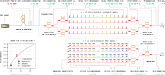
\includegraphics[width=0.85\textwidth]{fig/budget.pdf}}%
    \note<1-1>[item]{Now, let me have a few words on the energy efficiency of the link.}
    \note<2-2>[item]{And this energy estimation really starts from doing a link budget analysis, where I calculate the minimum power required from the comb laser to achieve a target bit error rate, which is 10 to the minus 12. This optical power from the comb will need to traverse a series of optical losses and eventually satisfy the receiver sensitivity.}
    \note<2-2>[item]{And I'd point out that all the optical losses listed here are characterized from measurement data.}

\end{frame}

\subsection{Breakdown}

\begin{frame}{Energy Breakdown}

    \only<1-1>{\centering\includegraphics[width=\textwidth]{fig/energy_compressed.pdf}}%
    \note<1-1>[item]{And then, the laser power consumption is calculated assuming a 15\% wall-plug efficiency, and the total energy consumption here includes not only the laser, but also the driver, receiver, and the thermal control. And it takes about 300 fJ/b with thermal undercut, which is foundry process that selectively removes part of the substrate around and below a device to improve the thermal tuning efficiency. And I'd like to emphasize that this 300 fJ/b is able to carry that data to almost any distance in the system.}

\end{frame}

\subsection{Further Improvement}
\begin{frame}{Return to Metrics}

    \only<1-1|handout:0>{\centering\includegraphics[width=0.8\textwidth]{fig/fom-5_compressed.pdf}}%
    \only<2-2>{\centering\includegraphics[width=0.8\textwidth]{fig/fom-future_compressed.pdf}}%
    \note<1-1>[item]{Now, let me return to this link metric and look at what we have achieved so far, and ask if we can further improve the bandwidth density and energy efficiency.}
    \note<2-2>[item]{And I'd say yes, at least another magnitude, and this is just the beginning, because we have lots of room to improve at both device and integration levels, like for example,}

\end{frame}

\begin{frame}{Paths to Improvement}

    \only<1-1|handout:0>{\centering\includegraphics[width=0.8\textwidth]{fig/path-improve-1_compressed.pdf}}%
    \only<2-2|handout:0>{\centering\includegraphics[width=0.8\textwidth]{fig/path-improve-2_compressed.pdf}}%
    \only<3-3>{\centering\includegraphics[width=0.8\textwidth]{fig/path-improve-3_compressed.pdf}}%
    \note<1-1>[item]{we have disk designs that can be driven faster at an even lower Vpp.}
    \note<2-2>[item]{Our link architecture is very scalable, and I'm working on characterizing this 4 by 32 transmitter array which has this disk design. So that'll be 128 channels at 32 Gb/s, or 4 Tb/s per fiber.}
    \note<3-3>[item]{And also with foundries starting to offer thick silicon nitride layers, we can potentially have an integrated comb source that lowers the optical losses and the energy consumption.}
    \note<3-3>[item]{And this is just the beginning because, as we start to think about a package like this, where it has an integrated comb source, and perhaps the photonics are directly driven by the compute or memory chip, there is a huge space for collaboration, with all the talks about heterogeneous integration and advanced packaging, that in addition to only electronic-photonic integration, how can we make a system with more chiplets integrated on an even larger substrate to further improve the system capabilities.}
    \note<3-3>[item]{With that, I would like to switch gears now and talk about how}

\end{frame}

%!TEX root = ../research_overview.tex

\section{Compute within Data Movement}

\subsection{Unified Interface}

\begin{frame}{Photonics-Enabled Data Processing}

    \only<1-1|handout:0>{\centering\includegraphics[width=\textwidth]{fig/pho-comp-1.pdf}}%
    \only<2-2>{\centering\includegraphics[width=\textwidth]{fig/pho-comp-2.pdf}}%
    \note<1-1>[item]{I extended this integrated photonics platform beyond classical data communications into the realm of computing accelerators.}
    \note<2-2>[item]{The goal here is to perform some data processing operations right at where the data resides.}
    \note<2-2>[item]{And, by having this unified photonic chiplet that can perform both data movement and data processing, we can reduce the need for shuttling data back and forth between the processor and the memory, but also be able to provide the high bandwidth when it is really needed.}


\end{frame}

\subsection{Photonic MAC}

\begin{frame}{Photonic Multiply-Accumulate (MAC) Accelerators}

    \only<2-2>{\centering\includegraphics[width=0.4\textwidth]{fig/matrix_compressed.pdf}}%
    \note<1-1>[item]{I'll give one example of my research in this direction, which is a photonic multiply-accumulate engine, or photonic MAC.}
    \note<2-2>[item]{Because MAC operations are essential for matrix multiplication, which is widely found in AI/machine learning and digital signal processing applications, it has drawn great attention for making accelerators for these operations, including using integrated photonics.}
    \note<2-2>[item]{And, this work that I'm going to talk about, differs from those existing photonic MAC engines by preserving the full digital precision of the MAC operation. And I'll show you how.}

\end{frame}

\begin{frame}{Existing Solutions Limited in Bit Precision}
    \only<1-1|handout:0>{\centering\includegraphics[width=0.9\textwidth]{fig/mac-limit-1_compressed.pdf}}%
    \only<2-2|handout:0>{\centering\includegraphics[width=0.9\textwidth]{fig/mac-limit-2_compressed.pdf}}%
    \only<3-3>{\centering\includegraphics[width=0.9\textwidth]{fig/mac-limit-3_compressed.pdf}}%
    \vspace{-1em}%
    \begin{center}%
        \fullcite{taitMicroringWeightBanks2016}%
    \end{center}%
    \note<1-1>[item]{Let's first take a look at a typical photonic MAC accelerator today using this architecture called a microring weight bank.}
    \note<2-2>[item]{Suppose we want to do a MAC operation like this. How this traditional architecture works is that, it encodes the multiplicand as an analog light intensity, and encodes the multiplier as an analog voltage applied to the microring, to control how much of a portion of that light can pass through.}
    \note<3-3>[item]{And as you may have noticed, this traditional approach requires converting these digitally stored numbers into the analog domain, and photonic devices aren't  actually good at precisely represent these analog values becaubese they're prone to fabrication and environmental perturbations. This limitation also applies to those architectures using a mesh of Mach-Zehnder interferometers, which encodes the numbers into an analog phase shift. And as a result, these methods are often limited in bit precision that they can achieve.}
\end{frame}

\begin{frame}{Photonic MAC with Full Digital Precision}

    \only<1-1|handout:0>{\centering\includegraphics[width=0.9\textwidth]{fig/dac-1_compressed.pdf}}%
    \only<2-2|handout:0>{\centering\includegraphics[width=0.9\textwidth]{fig/dac-2_compressed.pdf}}%
    \only<3-3|handout:0>{\centering\includegraphics[width=0.9\textwidth]{fig/dac-3_compressed.pdf}}%
    \only<4-4>{\centering\includegraphics[width=0.9\textwidth]{fig/dac-4_compressed.pdf}}%
    \vspace{0.25em}%
    \begin{center}%
        \onslide<1->{\tiny Nauman, N., Robinson, J., \textbf{Wang, Y.} \emph{et al.} in \emph{OFC}, (2025)}%
    \end{center}%
    \note<1-1>[item]{What's unique about our approach is that, we operate the photonic devices in the digital domain.}
    \note<2-2>[item]{And, leveraging our capability of having massive wavelengths channels, we directly look at each bit place of the MAC operation, and assign each digit contributing to this bit place a unique wavelength.}
    \note<3-3>[item]{Now, to get the MAC result of this bit place becomes counting the number of ones on this bus, where a one would let the light pass and a zero would block the light. So, this counting can be performed instantaneously by this analog photodetector at the end of this bus waveguide.}
    \note<3-3>[item]{This is where the acceleration comes from, because, we don't need to rely on using a bunch of adders to do the counting, so basically the larger the operation, the better gain in acceleration we can get.}
    \note<3-3>[item]{And this is why this architecture is uniquely enabled by our Kerr-comb driven DWDM, where we can have a large number of wavelength channels for this bit counting.}
    \note<4-4>[item]{And here I'm showing some experimental results from a bus waveguide with 8 microrings, and we can see that, since we are operating the microrings in a digital fashion, the output from this analog PD is really distinctive for different number of ones that are being counted.}

\end{frame}

\begin{frame}{Photonic ADC for MAC Result}

    \only<1-1|handout:0>{\centering\includegraphics[width=0.9\textwidth]{fig/adc-1_compressed.pdf}}%
    \only<2-2>{\centering\includegraphics[width=0.9\textwidth]{fig/adc-2_compressed.pdf}}
    \vspace{-1em}%
    \begin{center}%
        \onslide<1->{\tiny Nauman, N., Robinson, J., \textbf{Wang, Y.} \emph{et al.} in \emph{OFC}, (2025)}%
    \end{center}%
    \note<1-1>[item]{So the next step is to convert this analog PD output back into digital domain. And the least significant bit of the result will be the MAC output for this bit place, and the more significant bits will be the carry bits to higher bit places. And we can also do this in the optical domain, reusing this DWDM bus architecture.}
    \note<2-2>[item]{So, by biasing each of these microrings incrementally away from their resonance wavelengths, this same voltage applied to them will only flip a subset of the microrings, like shown in this plot, depending on the input voltage level. This is essentially doing a discretization of the input voltage using a cascaded microring bus.}
    \note<2-2>[item]{So this architecture really keeps both the input and output of the MAC operation in the digital domain while delegating the job of keeping the bit precision to leveraging more parallel wavelengths.}

\end{frame}

\subsection{Continued Scaling}

\begin{frame}{AI Scaling while Bending the Energy Curve}
    \only<1-1|handout:0>{\centering\includegraphics[width=0.75\textwidth]{fig/scaling-bend-1.pdf}}%
    \only<2-2>{\centering\includegraphics[width=0.75\textwidth]{fig/scaling-bend-2.pdf}}%
    \note<1-1>[item]{So, a quick summary, by empowering computing systems with both efficient data movement and data processing acceleration,}
    \note<2-2>[item]{my research aims to provide a mechanism to continue the scaling of AI computation, but at the same time, bending the energy curve, through the use of integrated photonics.}

\end{frame}

%!TEX root = ../research_overview.tex

\section{Future Directions}

\subsection{Photonics for RF}

\begin{frame}{Photonics-Enabled Massive Antenna Arrays}

    \only<2-2|handout:0>{\centering\includegraphics[width=0.8\textwidth]{fig/rf-1_compressed.pdf}}%
    \only<3-3>{\centering\includegraphics[width=0.8\textwidth]{fig/rf-2_compressed.pdf}}%
    \note<1-1>[item]{So, looking into the future, one exciting direction I would like to pursue is to find more applications of integrated photonics technology at the intersection of communication and computation.}
    \note<2-2>[item]{For example, for next-G wireless networks, massive distributed antenna arrays will be a key technology to provide both the high bandwidth and high angular resolution at the same time. And it requires ultra high-throughput signal processing and low-latency communication at the antenna backend.}
    \note<2-2>[item]{So, we can imagine having an RF antenna element directly interfaced with a photonic chip that can perform high-performance data processing locally,}
    \note<3-3>[item]{but can also communication with other elements through high-bandwidth optical interconnects and switches.}
    \note<3-3>[item]{This would open up the possibility of having, perhaps, a million-element antenna array in the future.}

\end{frame}

\subsection{3D Photonics}

\begin{frame}{3D Photonics for Transformative System Connectivity}

    \only<2-2|handout:0>{\centering\includegraphics[width=\textwidth]{fig/3d-1_compressed.pdf}}%
    \only<3-3>{\centering\includegraphics[width=\textwidth]{fig/3d-2_compressed.pdf}}%
    \note<1-1>[item]{Another exciting direction that I want to pursue is to explore the possibility of 3D optical routing and interconnections.}
    \note<2-2>[item]{This is really to break away from today's limitations of planar optical routing where every photonic component or waveguide needs to be on the same plane. And the bandwidth density you can have out of a chip is fundamentally limited by the fiber pitch you can have along a two dimensional shoreline.}
    \note<3-3>[item]{So, if we can route optical signals in the third dimension, and have dense optical I/Os that are accessible from essentially all directions, we would be able to transform the paradigm of optically connected systems, which currently relies on optical fibers, to something that uses an interposer-like photonic substrate.}
    \note<3-3>[item]{And this would potentially enable wafer-scale or panel-scale computation where each wafer or panel-sized system is capable of what a supercomputer can do today.}
    % \note<3-3>[item]{And I look forward to, and think that I would highly benefit from, collaborating with the faculty here who are experts in circuit design, such as Professor Kim and Professor Harjani, to explore electronic-photonic co-design and integration; and with top system architects, such as Professor Cao}


\end{frame}

\section{Acknowledgements}

\begin{frame}{Collaborators and Funding}
    \centering\includegraphics[width=\textwidth]{fig/ack_compressed.pdf}
    \large yw3831@columbia.edu
    \note[item]{And with that, I would like to thank you all for your attention, and I'm happy to take any questions.}
\end{frame}

\end{document}
